% Generated by Sphinx.
\documentclass[letterpaper,10pt,english]{manual}
\usepackage[utf8]{inputenc}
\usepackage[T1]{fontenc}
\usepackage{babel}
\usepackage{times}
\usepackage[Bjarne]{fncychap}
\usepackage{longtable}
\usepackage{sphinx}


\title{Odysseus Documentation}
\date{September 16, 2009}
\release{0.6.0}
\author{Ralf Gommers}
\newcommand{\sphinxlogo}{}
\renewcommand{\releasename}{Release}
\makeindex
\makemodindex
\newcommand\at{@}
\newcommand\lb{[}
\newcommand\rb{]}
\newcommand\PYGaz[1]{\textcolor[rgb]{0.00,0.63,0.00}{#1}}
\newcommand\PYGax[1]{\textcolor[rgb]{0.84,0.33,0.22}{\textbf{#1}}}
\newcommand\PYGay[1]{\textcolor[rgb]{0.00,0.44,0.13}{\textbf{#1}}}
\newcommand\PYGar[1]{\textcolor[rgb]{0.73,0.38,0.84}{#1}}
\newcommand\PYGas[1]{\textcolor[rgb]{0.25,0.44,0.63}{\textit{#1}}}
\newcommand\PYGap[1]{\textcolor[rgb]{0.00,0.44,0.13}{\textbf{#1}}}
\newcommand\PYGaq[1]{\textcolor[rgb]{0.38,0.68,0.84}{#1}}
\newcommand\PYGav[1]{\textcolor[rgb]{0.00,0.44,0.13}{\textbf{#1}}}
\newcommand\PYGaw[1]{\textcolor[rgb]{0.13,0.50,0.31}{#1}}
\newcommand\PYGat[1]{\textcolor[rgb]{0.73,0.38,0.84}{#1}}
\newcommand\PYGau[1]{\textcolor[rgb]{0.32,0.47,0.09}{#1}}
\newcommand\PYGaj[1]{\textcolor[rgb]{0.00,0.44,0.13}{#1}}
\newcommand\PYGak[1]{\textcolor[rgb]{0.14,0.33,0.53}{#1}}
\newcommand\PYGah[1]{\textcolor[rgb]{0.00,0.13,0.44}{\textbf{#1}}}
\newcommand\PYGai[1]{\textcolor[rgb]{0.73,0.38,0.84}{#1}}
\newcommand\PYGan[1]{\textcolor[rgb]{0.13,0.50,0.31}{#1}}
\newcommand\PYGao[1]{\textcolor[rgb]{0.25,0.44,0.63}{\textbf{#1}}}
\newcommand\PYGal[1]{\colorbox[rgb]{1.00,0.94,0.94}{\textcolor[rgb]{0.25,0.50,0.56}{#1}}}
\newcommand\PYGam[1]{\textbf{#1}}
\newcommand\PYGab[1]{\textit{#1}}
\newcommand\PYGac[1]{\textcolor[rgb]{0.25,0.44,0.63}{#1}}
\newcommand\PYGaa[1]{\textcolor[rgb]{0.19,0.19,0.19}{#1}}
\newcommand\PYGaf[1]{\textcolor[rgb]{0.25,0.50,0.56}{\textit{#1}}}
\newcommand\PYGag[1]{\textcolor[rgb]{0.13,0.50,0.31}{#1}}
\newcommand\PYGad[1]{\textcolor[rgb]{0.00,0.25,0.82}{#1}}
\newcommand\PYGae[1]{\textcolor[rgb]{0.13,0.50,0.31}{#1}}
\newcommand\PYGaZ[1]{\textcolor[rgb]{0.02,0.16,0.45}{\textbf{#1}}}
\newcommand\PYGbf[1]{\textcolor[rgb]{0.44,0.63,0.82}{\textit{#1}}}
\newcommand\PYGaX[1]{\textcolor[rgb]{0.00,0.44,0.13}{#1}}
\newcommand\PYGaY[1]{\textcolor[rgb]{0.25,0.44,0.63}{#1}}
\newcommand\PYGbc[1]{\textcolor[rgb]{0.25,0.44,0.63}{#1}}
\newcommand\PYGbb[1]{\textcolor[rgb]{0.78,0.36,0.04}{#1}}
\newcommand\PYGba[1]{\textcolor[rgb]{0.00,0.00,0.50}{\textbf{#1}}}
\newcommand\PYGaR[1]{\textcolor[rgb]{0.13,0.50,0.31}{#1}}
\newcommand\PYGaS[1]{\textcolor[rgb]{0.73,0.38,0.84}{#1}}
\newcommand\PYGaP[1]{\textcolor[rgb]{0.78,0.36,0.04}{\textbf{#1}}}
\newcommand\PYGaQ[1]{\textcolor[rgb]{0.25,0.44,0.63}{#1}}
\newcommand\PYGaV[1]{\textcolor[rgb]{0.05,0.52,0.71}{\textbf{#1}}}
\newcommand\PYGaW[1]{\textcolor[rgb]{0.25,0.44,0.63}{#1}}
\newcommand\PYGaT[1]{\textcolor[rgb]{0.13,0.50,0.31}{#1}}
\newcommand\PYGaU[1]{\textcolor[rgb]{0.25,0.50,0.56}{\textit{#1}}}
\newcommand\PYGaJ[1]{\textcolor[rgb]{0.56,0.13,0.00}{#1}}
\newcommand\PYGaK[1]{\textcolor[rgb]{0.25,0.44,0.63}{#1}}
\newcommand\PYGaH[1]{\textcolor[rgb]{0.50,0.00,0.50}{\textbf{#1}}}
\newcommand\PYGaI[1]{\fcolorbox[rgb]{1.00,0.00,0.00}{1,1,1}{#1}}
\newcommand\PYGaN[1]{\textcolor[rgb]{0.00,0.44,0.13}{#1}}
\newcommand\PYGaO[1]{\textcolor[rgb]{0.05,0.52,0.71}{\textbf{#1}}}
\newcommand\PYGaL[1]{\textcolor[rgb]{0.02,0.16,0.49}{#1}}
\newcommand\PYGaM[1]{\textcolor[rgb]{0.73,0.73,0.73}{#1}}
\newcommand\PYGaB[1]{\textcolor[rgb]{0.25,0.44,0.63}{#1}}
\newcommand\PYGaC[1]{\textcolor[rgb]{0.33,0.33,0.33}{\textbf{#1}}}
\newcommand\PYGaA[1]{\textcolor[rgb]{0.00,0.44,0.13}{#1}}
\newcommand\PYGaF[1]{\textcolor[rgb]{0.63,0.00,0.00}{#1}}
\newcommand\PYGaG[1]{\textcolor[rgb]{1.00,0.00,0.00}{#1}}
\newcommand\PYGaD[1]{\textcolor[rgb]{0.00,0.44,0.13}{\textbf{#1}}}
\newcommand\PYGaE[1]{\textcolor[rgb]{0.25,0.50,0.56}{\textit{#1}}}
\newcommand\PYGbg[1]{\textcolor[rgb]{0.00,0.44,0.13}{\textbf{#1}}}
\newcommand\PYGbe[1]{\textcolor[rgb]{0.00,0.44,0.13}{#1}}
\newcommand\PYGbd[1]{\textcolor[rgb]{0.40,0.40,0.40}{#1}}
\newcommand\PYGZat{@}
\newcommand\PYGZlb{[}
\newcommand\PYGZrb{]}

\begin{document}

\maketitle
\tableofcontents
\hypertarget{--doc-index}{}


Odysseus was started to have a complete, well-documented program to fit images of ultra-cold atom clouds. It has grown over time, so it now includes a graphical user interface that enables live image viewing and data analysis while running an experiment.

Odysseus is written in \href{http://python.org}{Python} and makes use of the \href{http://scipy.org/NumPy}{Numpy}, \href{http://scipy.org/}{Scipy} and \href{http://matplotlib.sourceforge.net/}{Matplotlib} packages. Most of the functionality is for fermionic atoms.


\chapter{Odysseus documentation contents}

\resetcurrentobjects
\hypertarget{--doc-introduction}{}

\section{Introduction}

Odysseus consists of a library of functions for analyzing data from cold-atom experiments and a graphical user interface (GUI) to these functions. In this section we will discuss what is needed to get Odysseus working, and the basics of using the GUI and library.


\subsection{Prerequisites}

Odysseus is written in \href{http://python.org}{Python} and requires a few Python libraries to run. The most important ones are \href{http://scipy.org/NumPy}{Numpy} (for fast numerics), \href{http://scipy.org/}{Scipy} (for fitting routines etc) and \href{http://matplotlib.sourceforge.net/}{Matplotlib} (for plotting). On Windows, a fully functional environment can be obtained simply by installing the \href{http://enthought.com/products/epd.php}{Enthought Python Distribution} and \href{http://www.riverbankcomputing.co.uk/software/pyqt/download}{PyQt4}. \href{http://www.sagemath.org/}{Sage} should work as well, but this has not yet been tested. On Linux, all libraries can be installed through the package manager on the most common distributions. This is all free software, so no license headaches.


\subsection{The GUI}

The GUI is straightforward to use, and allows new users to fit data with a number of functions without writing and scripts. It is also very useful to view images the moment they are acquired during an experimental run, and do some immediate analysis. The GUI is displayed below. For a detailed description of the functionality see the \hyperlink{section-gui}{\emph{section on the GUI}}.
\includegraphics[width=500pt]{odysseusgui.png}

\subsection{Writing analysis scripts}

The most efficient way of using Odysseus for analyzing a larger number of files is to write small scripts, that define the images you want to fit, and then to run these scripts from the command line. Standard Python works fine, but nicer is to use the \href{http://ipython.scipy.org/moin/}{IPython} interpreter. IPython and a nice editor of your choice can be used in the same way as you would use Matlab for interactive data analysis. A typical interactive session looks like this:
\includegraphics[width=500pt]{interactive_python.jpg}
In order to be able to run data analysis scripts from any directory, it is essential that the Python interpreter knows where to find the Odysseus modules. This requires setting the environment variable PYTHONPATH to include the Odysseus directory. For Windows XP this can be done via \emph{My Computer \textgreater{} Properties \textgreater{} Advanced (tab) \textgreater{} Environment Variables} and on Linux by defining PYTHONPATH in a shell startup rc file (.bashrc for example). To make sure this worked you can type \code{echo \$PYTHONPATH} in a terminal.


\subsection{Fitting an image}

Once everything is set up we can test if it all works. To do this we need the example script below and an image. Both can be found in the Odysseus source directory.

\begin{Verbatim}[commandchars=@\[\],numbers=left,firstnumber=1,stepnumber=1]
@PYGay[import] @PYGaV[os]
@PYGay[from] @PYGaV[odysseus.fitfermions] @PYGay[import] fit@_img

@PYGaE[@#dirname = '../../../archives/2008-05-27/']
dirname @PYGbd[=] @PYGaB[']@PYGaB[c:]@PYGao[\\]@PYGaB[Data]@PYGao[\\]@PYGaB[2008-05-27]@PYGaB[']

@PYGaE[@#@# this is how to fit a single image @#@#]
fname @PYGbd[=] @PYGaB[']@PYGaB[6msTOF.TIF]@PYGaB[']
img@_name @PYGbd[=] os@PYGbd[.]path@PYGbd[.]join(dirname, fname)
fit@_img(img@_name, odmax@PYGbd[=]@PYGaw[1.2], showfig@PYGbd[=]@PYGaA[True])
\end{Verbatim}

Open a terminal, go to the Odysseus source directory and start ipython there (simply type ``ipython -pylab'' at the promt and press enter. Then run the script by typing ``run example\_fit.py''.


\subsection{The structure of Odysseus}

Here is a visual representation of the structure of the code. Higher levels depend on lower levels but not the other way around, i.e. blue modules have no dependencies on other Odysseus code.
\includegraphics[width=500pt]{dependency_graph.png}
\resetcurrentobjects
\hypertarget{--doc-gui}{}

\hypertarget{section-gui}{}\section{The Graphical User Interface}

The graphical user interface (GUI) has two uses. One is to view images and get live feedback from fitting them when running an experiment. The other is to apply standard data analysis functions to single images without having to write analysis scripts. This section will describe the elements of the GUI in detail.


\subsection{Overview}

Here is an image of the GUI with images loaded, regions of interest and cursor displayed, and a temperature fit to the last image. The GUI is basically divided into three areas - central image view, image history and info panel. The GUI elements are discussed in later subsections.
\includegraphics[width=500pt]{odysseusgui.png}

\subsection{Image types}

Several image formats can be used for import and export. The main type, used by both Winview and XCamera, is TIFF. This is a very common bitmap format for scientific images. Unfortunately the 16-bit version is broken in both Python and C\#, therefore it is recommended to use 32-bit files. XCamera outputs 24-bit color files with a special structure that can be decoded by Odysseus. For more details see the documentation in the \emph{imageio} module.

In addition to TIFF Odysseus can import .xraw files, which are basically ascii files, and hdf5. There is ascii, npy (binary Numpy format) and hdf5 export available, and the images in the central image view can be saved as png, jpg, etc. For best interoperability one should use the hdf5 format, as it is the most commonly used standard scientific data format and can be read by Matlab, Mathematica, and most other program a scientist cares about.


\subsection{Data path}

This path is the one that is monitored by Odysseus for new files. If new files are detected they will be opened and the most recent one loaded into the central image view. Note that if the directory contains many Gb of image files the monitoring will get slower and start eating up more CPU time. It is therefore best to back up image files after a while and move them out of the monitored directory.


\subsection{Central image view}

The central image view contains an absorption image and all the raw frames used to calculate that absorption image. Typically these are `probe with atoms', `probe without atoms' and `dark field'. These can be viewed by clicking the + button on the top right corner of the view.

There are two regions of interest (ROIs), \emph{Analysis} and \emph{Ncount} that can be set by the respective control boxes on the right side of the GUI. The \emph{Analysis} ROI is used for fitting data and passing data to plugins, the \emph{Ncount} ROI for getting an estimate of the total number of atoms in the image. This \emph{ncount} number is shown below each image in the image history. Setting the ROI coordinates can be done by typing numbers in the spin boxes, or alternatively by right-clicking on the spin box labels. In the latter case the spin boxes will take the coordinate values of the cursor.

Right-clicking on the image will display the cursor at the point of the click. It can be moved around with the arrow keys. The coordinates and the image value are displayed in the light blue label above the image view. Right-clicking on that label will make the cursor disappear again.

At the bottom of the image view a row of buttons gives access to zoom levels and image saving. After activating the zoom functionality by clicking the button with the loupe, the image can be zoomed by left-dragging with the mouse. The arrow buttons and home button can be used to navigate back and forth through different zoom levels.


\subsection{Image history}

The row of images at the bottom of the GUI display the eight most recent images. Hovering the mouse over an image displays its file name in a tooltip. Left-clicking on an image loads it into the central image view, and right-clicking displays a list of plugins that can be invoked on the image.


\subsection{Fitting}

A large part of the Current Image Info panel on the right of the GUI is used for controlling and displaying fits of the image data. Selecting \emph{Autofit} automatically fits each loaded image with the selected function. If \emph{Calc ellipticity} is selected, the radial average that most fit functions perform takes into account that the image is stretched along the vertical axis. Select this option if you know your image is not radially symmetric, for example due to an inhomogeneous magnetic field that affects the cloud shape in time-of-flight.


\subsection{Plugins}

When right-clicking on an image in the history, a list of plugins is displayed. These plugins are a convenient way for users to add functionality without having to dig into the Odysseus source code. A simple format, documented in \hyperlink{writing-plugins}{\emph{writing plugins}}, allows one to write plain Python code assuming there is image data available under the variable \emph{img}. It can plot results in a pop-up window which the plugin system takes care of.

Useful plugins that are already available are, among others,:
* Line profile
* Radial average
* Fourier transform

\resetcurrentobjects
\hypertarget{--doc-theory}{}

\section{Theory}

The fitting procedure to extract the temperature from only the shape of the cloud seems to be most sensitive for temperatures between T/T\_F = 0.05 and T/T\_F = 0.4. For higher T/T\_F the cloud starts to resemble a Gaussian and for lower T/T\_F the differences become small because a smaller fraction of the atoms contributes to deviations in shape. In the figure below we can see the relative changes in shape for curves with different T/T\_F fitted to the same image.
\includegraphics[width=500pt]{fit_several_temperatures.png}

\subsection{Temperature fitting - dos and don'ts}

There are some things to keep in mind when you want a reliable temperature fit. First of all, it is very important that the image is as clean as possible (few fringes). This can be achieved by cleaning optical surfaces, by aperturing the imaging beam to limit backreflections, by angling optical surfaces, and by using a short optical path length after the imaging fiber.

Other things that can be done are:
\begin{itemize}
\item {} 
use a ROI with size at least two or three times the cloud size (otherwise we get normalization errors, or cut off significant parts of the data)

\item {} 
for a ROI, stay away from regions with no light and image edge by at least 10 pixels

\item {} 
use images with a central OD between \textasciitilde{} 0.6 and 1.6

\item {} 
results are not sensitive to TOF or cutoff OD when the above is done (check!)

\end{itemize}

\resetcurrentobjects
\hypertarget{--doc-fitfermions}{}

\section{User interface}

One of the goals of the development of Odysseus is to create an easy to use software package that fits images in a fast, simple and robust way. To achieve this, there is a single module, \code{fitfermions}, that contains high-level functions that can be used from user scripts. Most of the heavy lifting is being done by the function \code{fitfermions.fit\_img()}, which takes the path to a single image file, opens it, radially averages the transmission image, constructs the optical density profile, fits the column density for an ideal Fermi gas to it and finally extracts the number of atoms and temperature from the fit. Several example scripts are provided, they can be easily modified - with for example the names of the image files that are of interest - and run interactively.


\subsection{Example script}

Simply copy this script into a new file, modify and run!

\begin{Verbatim}[commandchars=@\[\],numbers=left,firstnumber=1,stepnumber=1]
@PYGay[import] @PYGaV[os]
@PYGay[from] @PYGaV[odysseus.fitfermions] @PYGay[import] fit@_img, find@_ellipticity
@PYGay[from] @PYGaV[odysseus.imageprocess] @PYGay[import] @PYGbd[*]
@PYGay[from] @PYGaV[odysseus.imageio] @PYGay[import] @PYGbd[*]

@PYGaE[@#@# import a single image @#@#]
dirname @PYGbd[=] @PYGaB[']@PYGaB[../../../archives/2008-09-11/]@PYGaB[']
@PYGaE[@#dirname = 'c:\\Data\\2008-05-27']
fname @PYGbd[=] @PYGaB[']@PYGaB[raw9.11.2008 7;35;23 PM.TIF]@PYGaB[']
img@_name @PYGbd[=] os@PYGbd[.]path@PYGbd[.]join(dirname, fname)

rawframes @PYGbd[=] import@_raw@_frames(img@_name)
transimg, odimg @PYGbd[=] calc@_absorption@_image(rawframes)
@PYGaE[@# set the ROI]
transimg @PYGbd[=] transimg@lb[]@PYGaw[120]:@PYGaw[350], @PYGaw[50]:@PYGaw[275]@rb[]

@PYGaE[@# find the ellipticity if the expansion is not spherically symmetric]
ellip @PYGbd[=] find@_ellipticity(transimg)
@PYGaE[@# do the fit]
ToverTF, N, ans @PYGbd[=] fit@_img(transimg, elliptic@PYGbd[=](ellip, @PYGaw[0]))
\end{Verbatim}

The above script results in the determined temperature and number of atoms being printed in the console, as well as an image containing the radially averaged transmission image, optical density profile and a fit of that OD profile with the expected one for an ideal Fermi gas, as shown below.
\includegraphics[width=400pt]{example_fit.png}

\subsection{The fitfermions module}
\index{odysseus.fitfermions (module)}
\hypertarget{module-odysseus.fitfermions}{}
\declaremodule[odysseus.fitfermions]{}{odysseus.fitfermions}
\modulesynopsis{}
A high level interface to the temperature fit routines for fermions.

The easiest to use function is fit\_img(). When a single transmission image
is passed in to this function, the fit should just work. Normalization
is automatically taken care of. It is assumed that the atom cloud is
azimuthally symmetric around its center of mass. If this is not the case,
find\_ellipticity() should be used to find the aspect ratio of the cloud first.
\index{fit\_img() (in module odysseus.fitfermions)}

\hypertarget{odysseus.fitfermions.fit_img}{}\begin{funcdesc}{fit\_img}{transimg, odmax=1.0, showfig=True, elliptic=None, pixcal=1.0000000000000001e-05, fitfunc='idealfermi', T=None, full\_output=None, norm=True}
Fits an absorption image with an ideal Fermi gas profile

The image is normalized, then azimuthally averaged, then fitted. If the
input is a list of imaged they are separately normalized and then averaged
and fitted.

\textbf{Inputs}
\begin{itemize}
\item {} 
transimg: 2D array or list of 2D arrays, containing the image data

\end{itemize}

\textbf{Outputs}
\begin{itemize}
\item {} 
ToverTF: float, the temperature of the Fermi gas in units of T\_F

\item {} 
N: float, the number of atoms of the Fermi gas

\end{itemize}

\textbf{Optional inputs}
\begin{itemize}
\item {} 
od\_max = float, the maximum optical density that is used in the fit

\item {} \begin{description}
\item[showfig: boolean, determines if a figure is shown with density profile] \leavevmode
and fit

\end{description}

\item {} 
elliptic: tuple, containing two elements. the first one is the
ellipticity (or ratio of major and minor axes), the second one is the
angle by which the major axis is rotated from the y-axis

\item {} 
pixcal: float, pixel size calibration in m/pix.

\item {} 
fitfunc: string, name of the fit function to be used. Valid choices are
idealfermi, gaussian, idealfermi\_fixedT

\item {} 
T: float, the temperature for idealfermi\_fixedT

\item {} 
full\_output: string, if value is \code{odysseus} the correct objects for
the Odysseus GUI are returned

\item {} \begin{description}
\item[norm: bool, if False the normalization of the image is turned off.] \leavevmode
This is mainly useful if you fit computer-generated images or
images that you already normalized some other way.

\end{description}

\end{itemize}
\end{funcdesc}
\index{norm\_and\_guess() (in module odysseus.fitfermions)}

\hypertarget{odysseus.fitfermions.norm_and_guess}{}\begin{funcdesc}{norm\_and\_guess}{transimg, norm=True}
Normalize the transmission image and find initial fitting parameters
\end{funcdesc}
\index{do\_fit() (in module odysseus.fitfermions)}

\hypertarget{odysseus.fitfermions.do_fit}{}\begin{funcdesc}{do\_fit}{rcoord, od\_prof, od\_cutoff, guess, pixcal, fitfunc='idealfermi', T=None}
Fits an absorption image with an ideal Fermi gas profile

\textbf{Inputs}
\begin{itemize}
\item {} 
rcoord: 1D array containing the radial coordinate

\item {} 
od\_prof: 1D array containing the radially averaged OD profile

\item {} \begin{description}
\item[od\_cutoff: int, the index of rcoord from where the fit has to be] \leavevmode
performed.

\end{description}

\item {} 
guess: tuple, initial fit parameters, the three elements are n0, a,
bprime

\item {} 
pixcal: float, pixel size calibration in m/pix.

\end{itemize}

\textbf{Outputs}
\begin{itemize}
\item {} 
ToverTF: float, the temperature of the Fermi gas in units of T\_F

\item {} 
N: float, the number of atoms of the Fermi gas

\item {} 
ans: tuple, containing the fit result

\end{itemize}

\textbf{Optional inputs}
\begin{itemize}
\item {} 
fitfunc: string, name of the fit function to be used. Valid choices are
idealfermi, gaussian, idealfermi\_fixedT

\item {} 
T: float, the temperature for idealfermi\_fixedT

\end{itemize}
\end{funcdesc}


\subsection{Sanity checks}

To make sure that fits make sense, a lot of tests can be done. There is a straightforward way to run many of these tests at once and generate a test report for an image. This comes in the form of a pdf file generated through LaTeX. In the simple example below an image is loaded, the region of interest (ROI) is set and a report generated.

\begin{Verbatim}[commandchars=@\[\],numbers=left,firstnumber=1,stepnumber=1]
@PYGay[import] @PYGaV[os]
@PYGay[from] @PYGaV[odysseus.imageprocess] @PYGay[import] @PYGbd[*]
@PYGay[from] @PYGaV[odysseus.imageio] @PYGay[import] @PYGbd[*]
@PYGay[from] @PYGaV[odysseus] @PYGay[import] texreport

dirname @PYGbd[=] @PYGaB[']@PYGaB[/home/ralf/data/archives/raw@_frames/]@PYGaB[']
tifname @PYGbd[=] @PYGaB[']@PYGaB[raw9.11.2008 7;35;23 PM.TIF]@PYGaB[']
imgname @PYGbd[=] os@PYGbd[.]path@PYGbd[.]join(dirname, tifname)

rawframes @PYGbd[=] import@_raw@_frames(imgname)
transimg, odimg @PYGbd[=] calc@_absorption@_image(rawframes)
transimg @PYGbd[=] transimg@lb[]@PYGaw[120]:@PYGaw[350], @PYGaw[50]:@PYGaw[275]@rb[] @PYGaE[@# ROI]
texreport@PYGbd[.]generate@_report(rawframes, transimg, imgname)
\end{Verbatim}

The transmission and raw images are shown, the azimuthally averaged image with the best fit is shown, the fit results (T, N) are given, the residuals are displayed, and the ellipticity is checked.

\resetcurrentobjects
\hypertarget{--doc-refimages}{}\index{odysseus.refimages (module)}
\hypertarget{module-odysseus.refimages}{}
\declaremodule[odysseus.refimages]{}{odysseus.refimages}
\modulesynopsis{Generating images from analytical expressions for density distributions}

\hypertarget{module-odysseus.refimages}{}\section{Generation of reference images}

We are interested in generating reference images from analytical expressions for the density distribution of atoms in a trap or in time-of-flight (TOF), in order to test our fit routines, get an idea of the effect of various types of noise, and to see for what experimental parameters we get useful data. We can generate transmission images, \emph{i.e. the same type of images we get from our experiment}, from either the fugacity, radial size and TOF or from T/T\_F, number of atoms and TOF.

To create an image we can do for example:

\begin{Verbatim}[commandchars=@\[\],numbers=left,firstnumber=1,stepnumber=1]
@PYGay[import] @PYGaV[odysseus.refimages] @PYGay[as] @PYGaV[refimg]

@PYGaE[@# T/T@_F = 0.1, N = 5e6, TOF = 3 ms]
central@_od, a, bprime @PYGbd[=] refimg@PYGbd[.]idealfermi@_fitparams(@PYGaw[0.1], @PYGaw[5e6], tof@PYGbd[=]@PYGaw[3e-3])
img @PYGbd[=] refimg@PYGbd[.]generate@_image(ODmax@PYGbd[=]central@_od, fugacity@PYGbd[=]a, cloudradius@PYGbd[=]bprime)
\end{Verbatim}

And then to plot the image:

\begin{Verbatim}[commandchars=@\[\],numbers=left,firstnumber=1,stepnumber=1]
@PYGay[import] @PYGaV[pylab]

fig1 @PYGbd[=] pylab@PYGbd[.]figure(@PYGaw[1])
ax1 @PYGbd[=] fig1@PYGbd[.]add@_subplot(@PYGaw[111])
ax1@PYGbd[.]imshow(img, cmap@PYGbd[=]pylab@PYGbd[.]cm@PYGbd[.]gray, vmin@PYGbd[=]@PYGaw[0], vmax@PYGbd[=]@PYGaw[1.35])
pylab@PYGbd[.]show()
\end{Verbatim}

This should give the following result:
\includegraphics[width=400pt]{refimg.png}

\subsection{Adding noise}

We can add various types of noise to an image with the \code{add\_noise} function:
\index{add\_noise() (in module odysseus.refimages)}

\hypertarget{odysseus.refimages.add_noise}{}\begin{funcdesc}{add\_noise}{img, ampl=0.050000000000000003, noisetype='random', fringeargs=None}
Noise is added to an image.

\textbf{Inputs}
\begin{itemize}
\item {} 
img: 2d array, containing image data

\item {} 
ampl: float, amplitude of the noise

\item {} 
noisetype: string, value can be one of
\begin{itemize}
\item {} 
`random', adds unbiased white noise

\item {} 
`linear\_x', adds a linear gradient along x from 0 to ampl

\item {} 
`linear\_y', adds a linear gradient along y from 0 to ampl

\item {} 
`fringes', adds fringes with parameters fringeargs

\end{itemize}

\item {} 
fringeargs: sequence, containing four values
\begin{itemize}
\item {} 
angle: float, angle of fringes in radians with respect to the x-axis

\item {} 
freq: float, frequency of the fringes in pixels\textasciicircum{}\{-1\}

\item {} 
pos: tuple, central position of the fringes with respect to the CoM

\item {} 
size: float, size of the Gaussian envelope of the fringes

\end{itemize}

\end{itemize}

\textbf{Outputs}
\begin{itemize}
\item {} 
img: 2d array, the input image with noise added to it

\end{itemize}
\end{funcdesc}

To generate random noise plus fringes we can for example do:

\begin{Verbatim}[commandchars=@\[\],numbers=left,firstnumber=1,stepnumber=1]
fringeargs @PYGbd[=] (np@PYGbd[.]pi@PYGbd[/]@PYGaw[3], @PYGaw[0.03], (@PYGaw[60], @PYGaw[50]), @PYGaw[70])
img2 @PYGbd[=] add@_noise(img, ampl@PYGbd[=]@PYGaw[0.1], noisetype@PYGbd[=]@PYGaB[']@PYGaB[fringes]@PYGaB['], fringeargs@PYGbd[=]fringeargs)
img2 @PYGbd[=] add@_noise(img2, ampl@PYGbd[=]@PYGaw[0.1], noisetype@PYGbd[=]@PYGaB[']@PYGaB[random]@PYGaB['])
\end{Verbatim}

This should give the following result:
\includegraphics[width=400pt]{noisy_image.png}

\subsection{Effects of noise on fit results}

It turns out that the fit results are quite sensitive to errors in normalization. A few percent one way or another in the tail of the radially averaged density profile can mimic the effect of quantum degeneracy or make it look like a very hot cloud. Ideally we want to make sure the density profile is really zero at the edge, and then normalize after radial averaging. When we have non-uniform normalization noise over the ccd then it becomes a tough problem of course.

Uniform white noise added to the transmission image does not seem to be that much of a problem, unless the amplitude becomes large (\textgreater{}5\%). The main effect is to reduce the optical density in the center of the cloud (if OD \textgreater{} 1.5), but this part of the density profile is not usually taken into account when fitting.
\hypertarget{radialaveraging-label}{}

\subsection{Validity of radial averaging}

We do the radial averaging by first finding the center of mass (CoM), then drawing circles around it, picking points on these circles and then determining the value of the image at each of those points by a bi-linear interpolation on the four pixels surrounding them. This procedure can be invalidated by either noise in the image or by the cloud not actually being radially symmetric. The latter can for example be caused by stray magnetic fields that influence the expansion out of an optical trap.

The purpose of the \code{lineprofiles()} function is to generate radial line profiles and compare those with the radially averaged profile we use for fitting. It can generate plots for the sum of differences between raw and averaged data as a function of angle, as shown below for a generated image with only random noise.
\includegraphics[width=400pt]{raderror_randomnoise.png}
The black data points represent negative sums, the white ones positive sums. There seem to be no systematics in the error sums, therefore we can conclude that radial averaging is a valid procedure for this image.

We can check the error sums for generated images with various types of noise, such as random noise, linear background slopes, fringes and combinations of all these. We find that without normalization with \code{normalize\_img()} the background slopes invalidate the radial averaging. With normalization we only have a problem when there are fringes that overlap with the atoms. This means it is important to clean up the imaging beam profile and use an aperture to select only the useful part of the beam.

Result for image with random noise, linear slopes and strong fringes partly overlapping the atoms:
\includegraphics[width=400pt]{raderror_allkindsofnoise.png}

\subsection{Elliptical averaging}

It turns out that at low temperatures and magnetic fields of around 560 G, the expansion of the atom cloud is slow enough that we can observe an asymmetry between the horizontal and vertical directions in the image. This is due to imperfections in the coils and to gravity, and leads to faster expansion in the vertical than in the horizontal direction. Therefore we need to average elliptically instead of radially. We can do this by specifying the \code{elliptic} parameter in \code{fit\_img()} or \code{radial\_interpolate()}. This has to be a tuple with two elements, the first gives the ellipticity (or aspect ratio) and the second the angle of the axes of the ellipse with respect to the image axes. The plots of residuals of radial profiles, as above, let us then determine the ellipticity with an accuracy of about 1\%.

\resetcurrentobjects
\hypertarget{--doc-plugins}{}

\hypertarget{writing-plugins}{}\section{The GUI plugin system}

Odysseus contains a very straightforward plugin system that allows users to add
their own data analysis functionality. Basically, what is needed is a plain text
file to register the plugin and a python file with the analysis code.
Users can then right-click on images in the image grid at the bottom of the GUI,
and select the plugin from a popup list. The image will be passed to the plugin,
where the results of the data analysis can be easily plotted in a popup window.

The plugin system is based on \href{http://yapsy.sourceforge.net/}{Yapsy}, for the
details of the design please check the documentation on the Yapsy wesite.


\subsection{Plugin info file format}

The plugin info file gathers, as its name suggests, some basic
information about the plugin. On one hand it gives crucial information
needed to be able to load the plugin. On the other hand it provided
some documentation like information like the plugin author's name and
a short description fo the plugin functionality. The info file
should have the extension \emph{.odysseus-plugin}.

Here is an example of what such a file should contain:

\begin{Verbatim}[commandchars=@\[\]]
@PYGZlb[]Core@PYGZrb[]
Name = Demo Plugin
Module = demo@_plugin

@PYGZlb[]Documentation@PYGZrb[]
Author = Ralf
Version = 0.1
Website = None
Description = A simple plugin useful for basic testing
\end{Verbatim}


\subsection{Plugin Python file}

The plugin should have extension \emph{.py} and contain a class that
is a subclass of DialogPlugin. The
\emph{main()} method of this class is executed when the plugin is used from the
GUI. Inside the \emph{main()} function a matplotlib figure and axes instance are
available as \emph{self.fig} and \emph{self.ax} respectively.

The following is an example of a basic plugin:

\begin{Verbatim}[commandchars=@\[\],numbers=left,firstnumber=1,stepnumber=1]
@PYGay[import] @PYGaV[numpy] @PYGay[as] @PYGaV[np]
@PYGay[from] @PYGaV[plugins] @PYGay[import] DialogPlugin

@PYGay[class] @PYGaO[DemoPlugin](DialogPlugin):
    @PYGas["""Demonstrates the basics of the plugin system"""]

    @PYGay[def] @PYGaL[main](@PYGaA[self], img):
        @PYGas["""Plot the average pixel intensity in each image row"""]

        x @PYGbd[=] np@PYGbd[.]arange(img@PYGbd[.]shape@lb[]@PYGaw[0]@rb[])
        y @PYGbd[=] img@PYGbd[.]mean(axis@PYGbd[=]@PYGaw[1])

        @PYGaA[self]@PYGbd[.]ax@PYGbd[.]plot(x, y)
\end{Verbatim}

The easiest thing to do is to copy the code above and simply change the contents
of the \emph{main()} function to something more useful.

\resetcurrentobjects
\hypertarget{--doc-development}{}

\section{Odysseus development}

This section describes the development of Odysseus itself. If all you want to do is use Odysseus to fit your data, you can skip this section.


\subsection{Organization of the code}

The way the code is organized is pretty much clear from the way the files are named. All functions used to fit optical density distributions live in \code{fitfuncs}. All code related to handling images - this includes reading/writing images, normalizing, smoothing, etc. - lives in the modules \code{imageio} and \code{imageprocess}. The main user interface, i.e. high-level functions like \code{fitfermions.fit\_img()}, is \code{fitfermions}. These files form the core of Odysseus, further there are some files to generate images and do consistency checks on the results. The user documentation is written in reStructuredText (reST), the source files live in the \emph{docs} directory and the html and pdf docs live under the .build directory.

Here is a visual representation of the source code. Higher levels depend on lower levels but not the other way around, i.e. blue modules have no dependencies on other Odysseus code.
\includegraphics[width=500pt]{dependency_graph.png}

\subsection{Documentation}

New code should be well-documented, no exceptions. All functions require docstrings in the following form

\begin{Verbatim}[commandchars=@\[\],numbers=left,firstnumber=1,stepnumber=1]
@PYGay[def] @PYGaL[function@_name](in1, in2, in3@PYGbd[=]@PYGaA[None]):
    @PYGas["""A one-line summary of what the function does, without func name in it]

@PYGas[    A paragraph with a more detailed explanation ...]

@PYGas[    **Inputs**]

@PYGas[      * in1: type(in1), is the independent variable]
@PYGas[      * in2: type(in2), is fit parameter with values between a and b]

@PYGas[    **Outputs**]

@PYGas[     * out1: etc]
@PYGas[     * out2: ...]

@PYGas[    **Optional inputs**]

@PYGas[     * in3: type(in3), this does ...]

@PYGas[    **References**]

@PYGas[    @lb[]1@rb[] Title, author, publication, year]

@PYGas[    """]
\end{Verbatim}

The one-line summary and lists of inputs/outputs are mandatory, the rest is optional. If significant new features are added, they should also be described in this documentation, which is generated with \href{http://sphinx.pocoo.org}{Sphinx}.

The documentation can be built with the Makefile in the source directory. For generating html use the command \code{make html} in that directory, for pdf use \code{make latex} in the source directory followed by \code{make all-pdf} in the directory \code{.build/latex/}.


\subsection{Tests}

The test coverage is not yet very good, but all new code should be covered by tests. Unit testing is done with the \href{http://somethingaboutorange.com/mrl/projects/nose/}{nose} testing framework. This should take care of low-level testing, i.e. if functions give the correct result for known inputs, and if they take the right parameters. All unit tests can be run by use of the command

\begin{Verbatim}[commandchars=@\[\]]
@$ nosetests
\end{Verbatim}

in the base directory of the code. For new code, a convenient way to stub out all the required unit tests is to run \href{http://pythoscope.org/}{Pythoscope}.

High level testing is done by running all the examples, with the \code{run\_examples.py} script.

To see which lines of a particular module are exercised by the tests, we can run \emph{nose} with the \href{http://somethingaboutorange.com/mrl/projects/nose/}{coverage.py} tool enabled:

\begin{Verbatim}[commandchars=@\[\]]
@$ nosetests --with-coverage --cover-package=polylog
\end{Verbatim}

This will typically result in output like this:

\begin{Verbatim}[commandchars=@\[\]]
Name      Stmts   Exec  Cover   Missing
---------------------------------------
polylog     107     45    42@%   81-108, 161-184, 190-193, 201-210, 216-225
----------------------------------------------------------------------
\end{Verbatim}


\subsection{Version control with Mercurial}

We use the distributed version control system \href{http://www.selenic.com/mercurial/wiki/}{Mercurial} for developing Odysseus. The basic idea is that each developer has his own brach(es) on his own computer, and when he/she completes a feature \emph{(that means including docstrings, documentation and ideally tests)} it is pushed to the central repository on Naboo. If it is something significant, please tell the other developers.

The basic workflow can look like this:

\begin{Verbatim}[commandchars=@\[\]]
@$ hg clone //naboo/personal/ralf/odysseus local@_repo
\end{Verbatim}

This gives you a local copy of the main repo. It is important to understand what effect the commands you use will have, therefore remember that \code{hg help} is your friend. To inspect the status of your files use the following commands on the command line

\begin{Verbatim}[commandchars=@\[\]]
@$ hg log
changeset:   43:7abaa4075238
tag:         tip
user:        Ralf Gommers @textless[]ralf.gommers@at[]googlemail.com@textgreater[]
date:        Tue Jun 10 02:39:48 2008 -0400
summary:     Finished up normalization and checks of radial profiles, including docstrings.
...

@$ hg status
M fitfuncs.py
M image@_treatment.py
M index.rst
M introduction.rst
? development.rst

@$ hg incoming
comparing with /home/ralf/smb4k/NABOO/PERSONAL/ralf/odysseus
searching for changes
no changes found
\end{Verbatim}

If there are changes in the main repo you can pull them into your local repo, and then merge those changes with the ones you made locally

\begin{Verbatim}[commandchars=@\[\]]
@$ hg pull //naboo/personal/ralf/odysseus
@$ hg merge
\end{Verbatim}

Then when all seems happy, commit your changes (with a good commit message describing what the hell everything does!) and push them to the main repo

\begin{Verbatim}[commandchars=@\[\]]
@$ hg commit
@$ hg push //naboo/personal/ralf/odysseus
\end{Verbatim}

For more details, please have a look at this \href{http://www.selenic.com/mercurial/wiki/index.cgi/Tutorial}{tutorial} and the rest on the information on the Mercurial site. Also, play with Mercurial a bit on your own computer before you try to push to the central repository!


\subsection{Debugging}

When there is a problem in a script, running it with IPython gives nicely color-coded tracebacks. These are usually good enough to tell you what the problem is. The Odysseus GUI catches a lot of exceptions to make sure that the whole program does not crash when for example a fit fails. Any exceptions that are not explicitly caught in the code generate a html log file in the directory \code{logs} in the source tree. These can be viewed with any browser.

\resetcurrentobjects
\hypertarget{--doc-imageprocess}{}

\section{Image handling}

All I/O related code, i.e. loading and saving, images lives in the \code{imageio} module. The code for processing images lives in \code{imageprocess}. Some functionality is independent of the type of image, for example smoothing, thresholding and interpolation. Other functionality is specific to cold atom experiments, for example calculating optical density and transmission for absorption images.
\index{odysseus.imageio (module)}
\hypertarget{module-odysseus.imageio}{}
\declaremodule[odysseus.imageio]{}{odysseus.imageio}
\modulesynopsis{}
I/O functions for several image formats.

The relevant formats are TIF, hdf5 and ascii. For ascii and binary numpy formats
no separate functions are provided for saving an image. This is because saving
in these formats requires just a single command:
ascii: np.savetxt(`filename', img)
binary (.npy): np.save(`filename', img)
\index{convert\_xcamera\_to\_hdf5() (in module odysseus.imageio)}

\hypertarget{odysseus.imageio.convert_xcamera_to_hdf5}{}\begin{funcdesc}{convert\_xcamera\_to\_hdf5}{imglist, ext='xraw'}
Convert every file in imglist to an hdf5 file.

The raw files are saved in the hdf5 file as
\emph{root.rawframes.pwa}, \emph{root.rawframes.pwoa}, \emph{root.rawframes.df}.
Their dtype is uint16, which results in files of a third smaller than
the xcamera text files.

\textbf{Inputs}
\begin{itemize}
\item {} 
imglist: list of str, paths to .xraw0 files

\item {} 
ext: str, the extension of the XCamera file. Normally xraw or xroi.

\end{itemize}
\end{funcdesc}
\index{imgimport\_intelligent() (in module odysseus.imageio)}

\hypertarget{odysseus.imageio.imgimport_intelligent}{}\begin{funcdesc}{imgimport\_intelligent}{img\_name}
Opens an image file containing one or more frames

The number of frames in the image is automatically detected. If it is a
single frame, it is assumed to be a transmission image. If there are three
frames, the first one is assumed to be probe with atoms (pwa), the second
one probe without atoms (pwoa) and the third one a dark field (df).
For four frames, it is assumed to be (pwoa, pwa, df1, df2).
For six frames, the first two are discarded (they are for clearing the
CCD charge on the Coolsnap camera), three to six are (pwoa, pwa, df1, df2).

\textbf{Inputs}
\begin{itemize}
\item {} 
img\_name: string containing the full path to an image

\end{itemize}

\textbf{Outputs}
\begin{itemize}
\item {} \begin{description}
\item[img\_array: 3D array, containing the three or four frames of the image,] \leavevmode
in the  order (pwa, pwoa, df, df2).

\end{description}

\end{itemize}

\textbf{Notes}

The datatype has to be set to float in Winview, otherwise there is a
strange problem reading the frames; support for 16-bit tif files is
lacking a bit in PIL. Note: when pil\_lite is available this does work.

The same support is lacking in MS .Net apparently, hence the weird check
for 3-channel TIFFs. What happens here is that XCamera can output multipage
8-bit RGB TIFFs. Each page is of shape (M,N,3), where the 8-bit color
channels combine to output 24-bit B/W data.
\end{funcdesc}
\index{import\_rawframes() (in module odysseus.imageio)}

\hypertarget{odysseus.imageio.import_rawframes}{}\begin{funcdesc}{import\_rawframes}{img\_name}
Opens an image file containing three frames

The datatype has to be set to float in Winview, otherwise there is a
strange problem reading the frames; support for 16-bit tif files is
lacking a bit in PIL.

\textbf{Inputs}
\begin{itemize}
\item {} 
img\_name: string containing the full path to an image

\end{itemize}

\textbf{Outputs}
\begin{itemize}
\item {} 
img\_array: 3D array, containing the three frames of the image

\end{itemize}
\end{funcdesc}
\index{import\_rawimage() (in module odysseus.imageio)}

\hypertarget{odysseus.imageio.import_rawimage}{}\begin{funcdesc}{import\_rawimage}{img\_name}
Opens an image file and returns it as an array.
\end{funcdesc}
\index{import\_xcamera() (in module odysseus.imageio)}

\hypertarget{odysseus.imageio.import_xcamera}{}\begin{funcdesc}{import\_xcamera}{img\_name, ext='xraw'}
Load the three .xraw files from XCamera

It is assumed that the file with extension .xraw0 contains the probe
with atoms (pwa), the one with extension .xraw1 the probe without atoms
(pwoa), and the one with extension .xraw2 the dark field (df).

\textbf{Inputs}
\begin{itemize}
\item {} \begin{description}
\item[img\_name: str, name of the image with or without extension] \leavevmode
(the extension is stripped and replaced by \emph{ext}.

\end{description}

\item {} 
ext: str, the extension of the XCamera file. Normally xraw or xroi.

\end{itemize}

\textbf{Outputs}
\begin{itemize}
\item {} 
raw\_array: 3D array, containing the three raw frames (pwa, pwoa, df)

\end{itemize}
\end{funcdesc}
\index{list\_of\_frames() (in module odysseus.imageio)}

\hypertarget{odysseus.imageio.list_of_frames}{}\begin{funcdesc}{list\_of\_frames}{img\_name}
Return the list of frames for an image file.

Details are as described in the imgimport\_intelligent docstring.
\end{funcdesc}
\index{load\_hdfimage() (in module odysseus.imageio)}

\hypertarget{odysseus.imageio.load_hdfimage}{}\begin{funcdesc}{load\_hdfimage}{fname, dirname=None, ext\_replace=True}
Load an image from an hdf5 file

\textbf{Inputs}
\begin{itemize}
\item {} \begin{description}
\item[fname: str, filename of the file to save, optionally including] \leavevmode
the full path to the directory

\end{description}

\item {} \begin{description}
\item[dirname: str, if not None, fname will be appended to dirname to] \leavevmode
obtain the full path of the file to save.

\end{description}

\item {} 
ext\_replace: bool, if True replaces the extension of fname with \emph{.h5}

\end{itemize}

\textbf{Outputs}
\begin{itemize}
\item {} 
transimg: ndarray, the image data

\end{itemize}
\end{funcdesc}
\index{save\_hdfimage() (in module odysseus.imageio)}

\hypertarget{odysseus.imageio.save_hdfimage}{}\begin{funcdesc}{save\_hdfimage}{imgarray, fname, dirname=None}
Save an image to an hdf5 file

\textbf{Inputs}
\begin{itemize}
\item {} \begin{description}
\item[imgarray: ndarray, containing the image data. If the array is 2D,] \leavevmode
it is assumed that this is a single frame image. If it is
3D, the frames will be saved as separate arrays:
(`pwa', `pwoa', `df'), and if there is a fourth frame this
is df2.

\end{description}

\item {} \begin{description}
\item[fname: str, filename of the file to save, optionally including] \leavevmode
the full path to the directory

\end{description}

\item {} \begin{description}
\item[dirname: str, if not None, fname will be appended to dirname to] \leavevmode
obtain the full path of the file to save.

\end{description}

\end{itemize}
\end{funcdesc}
\index{save\_tifimage() (in module odysseus.imageio)}

\hypertarget{odysseus.imageio.save_tifimage}{}\begin{funcdesc}{save\_tifimage}{imgarray, fname, dirname=None}
Save a single image in TIF format

\textbf{Inputs}
\begin{itemize}
\item {} 
imgarray: 2D array, containing a single frame image

\item {} \begin{description}
\item[fname: str, filename of the file to save, optionally including] \leavevmode
the full path to the directory

\end{description}

\item {} \begin{description}
\item[dirname: str, if not None, fname will be appended to dirname to] \leavevmode
obtain the full path of the file to save.

\end{description}

\end{itemize}

\textbf{Notes}

Multiple frame tif images are not supported. For such data hdf5 is the
recommended format.
\end{funcdesc}
\index{odysseus.imageprocess (module)}
\hypertarget{module-odysseus.imageprocess}{}
\declaremodule[odysseus.imageprocess]{}{odysseus.imageprocess}
\modulesynopsis{}
Image processing functions

Some functionality is independent of the type of image, for example
smoothing, thresholding and interpolation. Other functionality is specific
to cold atom experiments, for example calculating optical density and
transmission for absorption images.
\index{bilinear\_interpolate() (in module odysseus.imageprocess)}

\hypertarget{odysseus.imageprocess.bilinear_interpolate}{}\begin{funcdesc}{bilinear\_interpolate}{xr, yr, img}
Do a bi-linear interpolation to get the value at image coordinates
\begin{description}
\item[\textbf{Inputs}] \leavevmode\begin{itemize}
\item {} 
xr: array-like, the x-coordinates of the point to be interpolated

\item {} 
yr: array-like, the y-coordinates of the point to be interpolated

\item {} 
img: 2d-array, the image data

\end{itemize}

\item[\textbf{Outputs}] \leavevmode\begin{itemize}
\item {} 
ans: array-like, the result of the interpolation

\end{itemize}

\end{description}
\end{funcdesc}
\index{calc\_absimage() (in module odysseus.imageprocess)}

\hypertarget{odysseus.imageprocess.calc_absimage}{}\begin{funcdesc}{calc\_absimage}{raw\_frames, norm\_edge=False}
Calculates the transmission image and optical density.

\textbf{Inputs}
\begin{itemize}
\item {} \begin{description}
\item[raw\_frames: 3D array, containing three or four images;] \leavevmode
probe with atoms (pwa), probe without atoms (pwoa),
dark field (df) and \emph{optionally} a second dark field (df2).
If there is no second dark field, the same one is used
twice.

\end{description}

\item {} \begin{description}
\item[norm\_edge: bool, if True, normalize to one using the edge (it is assumed] \leavevmode
no atoms are visible on the edge.

\end{description}

\end{itemize}

\textbf{Outputs}
\begin{itemize}
\item {} \begin{description}
\item[transimg: 2d array containing the transmission image,] \leavevmode
defined as (pwa - df)/(pwoa - df2).

\end{description}

\item {} 
odimg: 2d array containing the optical density for each pixel

\end{itemize}
\end{funcdesc}
\index{find\_fitrange() (in module odysseus.imageprocess)}

\hypertarget{odysseus.imageprocess.find_fitrange}{}\begin{funcdesc}{find\_fitrange}{od\_prof, od\_max=1, min\_cutoff=8}
Select a suitable range of radii to use for fitting the image.

When the optical density saturates at a certain range of radii, and then
that data range is used for fitting, it throws off the fit. Therefore
a cutoff value for the maximum optical density should be specified, and the
fit only done for values of OD smaller than that. The data is smoothed,
and the index for the radius where the OD drops below OD\_max is determined.

\textbf{Inputs}
\begin{itemize}
\item {} \begin{description}
\item[od\_prof: 1D array, containing the radially averaged optical density] \leavevmode
profile.

\end{description}

\end{itemize}

\textbf{Outputs}
\begin{itemize}
\item {} \begin{description}
\item[cutoff: int, the larger value of index of rcoord where od\_prof\textless{}od\_max] \leavevmode
or min\_cutoff.

\end{description}

\end{itemize}

\textbf{Optional inputs}
\begin{itemize}
\item {} 
od\_max: float, the maximum desired value of the optical density

\item {} \begin{description}
\item[min\_cutoff: int, the minimum value for the cutoff index. The reason to] \leavevmode
use this is that a radially averaged profile is very noisy
around the center which may skew a fit.

\end{description}

\end{itemize}
\end{funcdesc}
\index{imgslice() (in module odysseus.imageprocess)}

\hypertarget{odysseus.imageprocess.imgslice}{}\begin{funcdesc}{imgslice}{img, cpoint, angle=0, width=None}
Take a line profile through the centerpoint
\begin{description}
\item[\textbf{Inputs}] \leavevmode\begin{itemize}
\item {} 
img: 2D array, the image data

\item {} 
cpoint: 1D array, the center point coordinates of the required slice

\end{itemize}

\item[\textbf{Outputs}] \leavevmode\begin{itemize}
\item {} 
lprof\_coord: 1D array, the slice indices in units of pixels

\item {} 
lprof: 1D array, the slice data

\end{itemize}

\end{description}

\textbf{Optional inputs}
\begin{itemize}
\item {} 
angle: float, the angle under which the slice is taken in degrees

\item {} 
width: float, the width over which the slice is averaged

\end{itemize}
\end{funcdesc}
\index{lineprofiles() (in module odysseus.imageprocess)}

\hypertarget{odysseus.imageprocess.lineprofiles}{}\begin{funcdesc}{lineprofiles}{img, com, rcoord, phi, elliptic=None}
Generate radial profiles around center of mass

Line profiles without any averaging are generated. This is useful for
comparing the radially averaged profile with, to make sure that that is a
valid procedure.

\textbf{Inputs}
\begin{itemize}
\item {} 
img: 2D array, normally containing image data

\item {} 
com: 1D array with two elements, the center of mass coordinates in pixels

\item {} \begin{description}
\item[rcoord: 1D array, radial coordinate for line profiles] \leavevmode
this is usually obtained from radial\_interpolate

\end{description}

\item {} 
phi: 1D array, angles along which line profiles are required

\end{itemize}

\textbf{Outputs}
\begin{itemize}
\item {} 
rprofiles: 2D array, containing radial profiles along angles

\end{itemize}

\textbf{Optional inputs}
\begin{itemize}
\item {} 
elliptic: tuple, containing two elements. the first one is the
ellipticity (or ratio of major and minor axes), the second one is the
angle by which the major axis is rotated from the y-axis. This should
be the same as used for radial averaging.

\end{itemize}

\textbf{Notes}
\begin{quote}

The form used for mapping an ellipse to (x,y) coordinates is:
x = acosphicoslpha - bsinphisinlpha
y = bsinphicoslpha + acosphisinlpha
\end{quote}
\end{funcdesc}
\index{maxod\_correct() (in module odysseus.imageprocess)}

\hypertarget{odysseus.imageprocess.maxod_correct}{}\begin{funcdesc}{maxod\_correct}{odimg, odmax}
Corrects calculated OD from an absorption image for finite OD\_max

This idea was taken from Brian DeMarco's thesis, but it does not seem to
make much of a difference at low OD. For high-OD images it causes errors
because there will be data points with measured OD higher than the maximum
observable OD due to noise in the image.

It is left in here for completeness, but it is recommended to not use this
method. Instead, images should be taken in a regime where this correction
is negligibly small anyway (i.e. below an OD of 1.5).
\end{funcdesc}
\index{mirror\_line() (in module odysseus.imageprocess)}

\hypertarget{odysseus.imageprocess.mirror_line}{}\begin{funcdesc}{mirror\_line}{linedata, negative\_mirror=False}
Mirrors a 1D array around its first element

\textbf{Inputs}
\begin{itemize}
\item {} 
linedata: 1D array, the array to be mirrored

\item {} \begin{description}
\item[negative\_mirror: bool, if True the mirrors elements are multiplied by] \leavevmode
-1. This is useful to mirror the x-axis of a plot.

\end{description}

\end{itemize}

\textbf{Outputs}
\begin{itemize}
\item {} \begin{description}
\item[mirrored: 1D array, the output array, which is now symmetric around its] \leavevmode
midpoint.

\end{description}

\end{itemize}
\end{funcdesc}
\index{normalize\_edgestrip() (in module odysseus.imageprocess)}

\hypertarget{odysseus.imageprocess.normalize_edgestrip}{}\begin{funcdesc}{normalize\_edgestrip}{img, normval=1.0, striplen=5}
Normalizes the image so the average value on the edges is normval.

This is simply a multiplication of the whole image array by a number
so that the average intensity on the edges of the image is \emph{normval}.

\textbf{Inputs}
\begin{itemize}
\item {} 
img: 2D array, image data

\item {} 
normval: float, the value to which img is normalized

\item {} 
striplen: int, number of pixels along each edge used for normalization

\end{itemize}

\textbf{Outputs}
\begin{itemize}
\item {} 
normimg: 2D array, the normalized image

\end{itemize}
\end{funcdesc}
\index{normalize\_img() (in module odysseus.imageprocess)}

\hypertarget{odysseus.imageprocess.normalize_img}{}\begin{funcdesc}{normalize\_img}{img, com, size}
Mask off the atoms, then fit linear slopes to the image and normalize

We assume that there are no atoms left outside 1.5 times the size. This
seems to be a reasonable assumption, it does not influence the result of
the normalization.

\textbf{Inputs}
\begin{itemize}
\item {} 
img: 2D array, containing the image

\item {} 
com: tuple, center of mass coordinates

\item {} 
size: float, radial size of the cloud

\end{itemize}

\textbf{Outputs}
\begin{itemize}
\item {} 
normimg: 2D array, the normalized image

\end{itemize}
\end{funcdesc}
\index{od2trans() (in module odysseus.imageprocess)}

\hypertarget{odysseus.imageprocess.od2trans}{}\begin{funcdesc}{od2trans}{odimg, maxod=3.5}
Calculates the transmission image from an optical density image

For pixels with strange values due to noise, replace the value of that pixel
by the maximum OD that can be experimentally measured.
\end{funcdesc}
\index{radial\_interpolate() (in module odysseus.imageprocess)}

\hypertarget{odysseus.imageprocess.radial_interpolate}{}\begin{funcdesc}{radial\_interpolate}{img, com, dr, phi=None, elliptic=None, full\_output=False}
Does radial averaging around the center of mass of the image.

Radial averaging of the image data on circles spaced by dr around the
center of mass. The number of points on each circle is dphi*sqrt(i+1),
with i the circle index. A bilinear interpolation method is used.

\textbf{Inputs}
\begin{itemize}
\item {} 
img: 2D array, normally containing image data

\item {} \begin{description}
\item[com: 1D array with two elements, the center of mass coordinates in] \leavevmode
pixels

\end{description}

\item {} 
dr: radial step size in pixels

\end{itemize}

\textbf{Outputs}
\begin{itemize}
\item {} 
rcoord: 1D array containing the radial coordinate

\item {} 
rad\_profile: 1D array containing the averaged profile

\end{itemize}

\textbf{Optional inputs}
\begin{itemize}
\item {} \begin{description}
\item[phi: 1D array, the angles along which line profiles are taken. More] \leavevmode
values in phi means a more precise radial average; default is
2*pi times the maximum radius in pixels

\end{description}

\item {} 
elliptic: tuple, containing two elements. the first one is the
ellipticity (or ratio of major and minor axes), the second one is the
angle by which the major axis is rotated from the y-axis.

\item {} 
full\_output: bool, selects whether rprofiles and phi are returned

\end{itemize}
\end{funcdesc}
\index{radialprofile\_errors() (in module odysseus.imageprocess)}

\hypertarget{odysseus.imageprocess.radialprofile_errors}{}\begin{funcdesc}{radialprofile\_errors}{odprofiles, angles, od\_prof, od\_cutoff, showfig=False, savefig\_name=None, report=True}
Calculate errors in radial profiles as a function of angle

\textbf{Inputs}
\begin{itemize}
\item {} 
odprofiles: 2D array, containing radial OD profiles along angles

\item {} \begin{description}
\item[angles: 1D array, angles at which radial profiles are taken] \leavevmode
(zero is postive x-axis)

\end{description}

\item {} 
od\_prof: 1D array, radially averaged optical density

\item {} 
od\_cutoff: integer, index of profiles at which maximum fit-OD is reached

\end{itemize}

\textbf{Outputs}
\begin{itemize}
\item {} 
av\_err: float, sum of absolute values of errors in errsum

\end{itemize}

\textbf{Optional inputs}
\begin{itemize}
\item {} \begin{description}
\item[showfig: bool, determines if a figure is shown with density profile] \leavevmode
and fit

\end{description}

\item {} 
report: bool, if True print the sums of the mean and rms errors

\item {} \begin{description}
\item[savefig\_name: string, if not None and showfig is True, the figure is] \leavevmode
not shown but saved as png with this string as filename.

\end{description}

\end{itemize}
\end{funcdesc}
\index{smooth() (in module odysseus.imageprocess)}

\hypertarget{odysseus.imageprocess.smooth}{}\begin{funcdesc}{smooth}{x, window\_len=10, window='hanning'}
Smooth the data using a window with requested size.

This method is based on the convolution of a scaled window with the signal.
The signal is prepared by introducing reflected copies of the signal
(with the window size) in both ends so that transient parts are minimized
in the begining and end part of the output signal.

Adapted from the Scipy Cookbook by Ralf Gommers.

\textbf{Inputs}
\begin{itemize}
\item {} 
x: 1D array, data that needs to be smoothed

\end{itemize}

\textbf{Outputs}
\begin{itemize}
\item {} 
x\_smooth: 1D array, the smoothed signal

\end{itemize}

\textbf{Optional inputs}
\begin{itemize}
\item {} 
window\_len: int, the size of the smoothing window

\item {} \begin{description}
\item[window: str, the type of window from `flat', `hanning', `hamming',] \leavevmode
`bartlett', `blackman'. A flat window will produce a
moving average smoothing.

\end{description}

\end{itemize}
\end{funcdesc}
\index{threshold\_image() (in module odysseus.imageprocess)}

\hypertarget{odysseus.imageprocess.threshold_image}{}\begin{funcdesc}{threshold\_image}{img, thres=0.5, below=True}
Returns a binary array (ones and zeros) depending on pixel values.

\textbf{Inputs}
\begin{itemize}
\item {} 
img: array, containing an image (also works for non-image data)

\item {} 
thres: scalar value, the threshold value

\item {} \begin{description}
\item[below: boolean value, True means that each element of img that is below] \leavevmode
thres gives a 1 in the thresholded image, and each element that
is above it a 0.

\end{description}

\end{itemize}

\textbf{Outputs}
\begin{itemize}
\item {} \begin{description}
\item[thres\_img: array, containing ones and zeros as a result of] \leavevmode
thresholding the input array.

\end{description}

\end{itemize}
\end{funcdesc}
\index{trans2od() (in module odysseus.imageprocess)}

\hypertarget{odysseus.imageprocess.trans2od}{}\begin{funcdesc}{trans2od}{transimg, maxod=3.5}
Calculates the optical density image from a transmission image

For pixels with strange values due to noise, replace the value of that pixel
by the maximum OD that can be experimentally measured.
\end{funcdesc}

\resetcurrentobjects
\hypertarget{--doc-fitfuncs}{}

\section{Fitting functions}

The fit functions for density profiles of atom clouds live in the \code{fitfuncs} module.
\index{odysseus.fitfuncs (module)}
\hypertarget{module-odysseus.fitfuncs}{}
\declaremodule[odysseus.fitfuncs]{}{odysseus.fitfuncs}
\modulesynopsis{}
Collection of functions that can be used to fit images of cold atom clouds.

\textbf{References}

{[}1{]} ``Making, probing and understanding ultracold Fermi gases'', W. Ketterle and
M. Zwierlein, arXiv:cond-mat/0801.2500 (2008)

{[}2{]} ``Making, probing and understanding Bose-Einstein condensates:, W. Ketterle,
D.S. Durfee and D.M. Stamper-Kurn, arXiv:cond-mat/9904034 (1999)
\index{fit1dfunc() (in module odysseus.fitfuncs)}

\hypertarget{odysseus.fitfuncs.fit1dfunc}{}\begin{funcdesc}{fit1dfunc}{func, xdata, ydata, guess, weights=None, params=None, tol=1e-08}
Convenience function to fit 1d data

Note that if the fitted data has no noise, the fit will sometimes return
2 or 3 for success, but this usually still means that the fit was successful.

\textbf{Inputs}
\begin{itemize}
\item {} \begin{description}
\item[func: function, the 1D function that has only xdata as an independent] \leavevmode
variable

\end{description}

\item {} 
xdata: 1D array, the independent variable of func

\item {} 
ydata: 1D array, the independent variable of func we're fitting

\item {} 
guess: sequence, the initial guess for the fit parameters of func

\end{itemize}

\textbf{Outputs}
\begin{itemize}
\item {} 
ans: sequence, the final fitting parameters

\end{itemize}

\textbf{Optional inputs}
\begin{itemize}
\item {} 
weights: 1D array, the weights of the data points

\item {} 
params: sequence, containing the other input parameters to func

\item {} 
tol: relative tolerance of the fitting routine

\end{itemize}
\end{funcdesc}
\index{fugacity\_from\_temp() (in module odysseus.fitfuncs)}

\hypertarget{odysseus.fitfuncs.fugacity_from_temp}{}\begin{funcdesc}{fugacity\_from\_temp}{ToverTF}
Finds the fugacity from the temperature by a minimization routine
\end{funcdesc}
\index{gaussian() (in module odysseus.fitfuncs)}

\hypertarget{odysseus.fitfuncs.gaussian}{}\begin{funcdesc}{gaussian}{r, n0, sigma}
1d radial column density of a gas with Gaussian profile

\textbf{Inputs}
\begin{itemize}
\item {} 
r: 1d array containing the radial coordinate

\item {} 
n0: float, central optical density

\item {} 
sigma: float, Gaussian width

\end{itemize}

\textbf{Outputs}
\begin{itemize}
\item {} 
coldensity: 1d array of the same length as r, containing the column density

\end{itemize}
\end{funcdesc}
\index{gaussian\_numbers() (in module odysseus.fitfuncs)}

\hypertarget{odysseus.fitfuncs.gaussian_numbers}{}\begin{funcdesc}{gaussian\_numbers}{fitparams, pixcal, sigma=None}
Determine T/T\_F and N for an ideal Fermi gas.

\textbf{Inputs}
\begin{itemize}
\item {} \begin{description}
\item[fitparams: list, the result of fitting the image with gaussian().] \leavevmode
fitparams is a list containing the central optical density,
and thermal radius of the cloud in pixels

\end{description}

\item {} 
pixcal: calibration for the camera in meters per pixel

\end{itemize}

\textbf{Outputs}
\begin{itemize}
\item {} 
N: number of atoms

\end{itemize}

\textbf{Optional inputs}
\begin{itemize}
\item {} \begin{description}
\item[sigma: photon absorption cross-section] \leavevmode
the default value is the resonant cross-section for 6Li

\end{description}

\end{itemize}
\end{funcdesc}
\index{ideal\_fermi\_numbers() (in module odysseus.fitfuncs)}

\hypertarget{odysseus.fitfuncs.ideal_fermi_numbers}{}\begin{funcdesc}{ideal\_fermi\_numbers}{fitparams, pixcal, sigma=None}
Determine T/T\_F and N for an ideal Fermi gas.

\textbf{Inputs}
\begin{itemize}
\item {} \begin{description}
\item[fitparams: the result of fitting the image with ideal\_fermi\_radial] \leavevmode
fitparams is a list containing the central optical density,
logarithm of the fugacity and thermal radius of the cloud in
pixels

\end{description}

\item {} 
pixcal: calibration for the camera in meters per pixel

\end{itemize}

\textbf{Outputs}
\begin{itemize}
\item {} 
ToverTF: temperature of the Fermi gas T/T\_F

\item {} 
N: number of atoms

\end{itemize}

\textbf{Optional inputs}
\begin{itemize}
\item {} \begin{description}
\item[sigma: photon absorption cross-section] \leavevmode
the default value is the resonant cross-section for 6Li

\end{description}

\end{itemize}
\end{funcdesc}
\index{ideal\_fermi\_radial() (in module odysseus.fitfuncs)}

\hypertarget{odysseus.fitfuncs.ideal_fermi_radial}{}\begin{funcdesc}{ideal\_fermi\_radial}{r, n0, q, r\_cloud}
1D radial column density of an ideal Fermi gas

The radial column density of an ideal Fermi gas around its center of mass.
This is usually obtained by radially averaging an image of the atom cloud
after time of flight from a trap with equal trap frequencies along both
image axes.

\textbf{Inputs}
\begin{itemize}
\item {} 
r: 1D array containing the radial coordinate

\item {} 
n0: central optical density

\item {} 
q: logarithm of the fugacity, q = mu*beta

\item {} \begin{description}
\item[r\_cloud: the radius of the atom cloud after expansion, in pixels.] \leavevmode
for low temperatures T/T\_F \textless{}\textless{} 1, this is equal to the
Fermi radius times the expansion factor, for high T/T\_F
to the thermal radius times the expansion factor.

\end{description}

\end{itemize}

\textbf{Outputs}
\begin{itemize}
\item {} \begin{description}
\item[coldensity: 1D array of the same length as r, containing the column] \leavevmode
density for the ideal Fermi gas

\end{description}

\end{itemize}

\textbf{References}

{[}1{]} Ketterle and Zwierlein, p.69, eq.65
\end{funcdesc}
\index{n2D\_radial() (in module odysseus.fitfuncs)}

\hypertarget{odysseus.fitfuncs.n2D_radial}{}\begin{funcdesc}{n2D\_radial}{r, oneDfunc, oneDparams}
2D density distribution used for determining the number of atoms.

This is a convenience function that takes a 1D function that depends on
radius, and multiplies it by 2*pi*r so it can be integrated over in 2D.

\textbf{Inputs}
\begin{itemize}
\item {} 
r: radial coordinate, this is the independent variable of oneDfunc

\item {} 
oneDfunc: function, the 1D function that depends only on r

\item {} \begin{description}
\item[oneDparams: sequence, a list or tuple containing the other input] \leavevmode
parameters to oneDfunc

\end{description}

\end{itemize}

\textbf{Outputs}
\begin{itemize}
\item {} 
twoDfunc: oneDfunc times 2*pi*r

\end{itemize}
\end{funcdesc}

\resetcurrentobjects
\hypertarget{--doc-othermodules}{}

\section{Other modules}

The smaller modules that are part of Odysseus and do not warrant a more extensive description (yet) are documented in this section.


\subsection{filetools}

This module contains a few convenience functions to work with the file system. String handling and interaction with the operating system is easy to do in Python, and processing directories of files (or selections out of them) can be done with the help of this module.
\index{odysseus.filetools (module)}
\hypertarget{module-odysseus.filetools}{}
\declaremodule[odysseus.filetools]{}{odysseus.filetools}
\modulesynopsis{}
Functions to easily process file names.
\index{find\_imgnames() (in module odysseus.filetools)}

\hypertarget{odysseus.filetools.find_imgnames}{}\begin{funcdesc}{find\_imgnames}{imglist, startstr, stopstr}
Finds names from imglist between startstr and stopstr in time-ordered way

\textbf{Inputs}
\begin{itemize}
\item {} 
imglist: list of str, containing paths of images on disc

\item {} \begin{description}
\item[startstr: str, part of the name of the oldest image by date that is] \leavevmode
wanted

\end{description}

\item {} \begin{description}
\item[stopstr: str, part of the name of the newest image by date that is] \leavevmode
wanted

\end{description}

\end{itemize}

\textbf{Outputs}
\begin{itemize}
\item {} 
imgs: list of str, containing the found paths to image files

\end{itemize}
\end{funcdesc}
\index{get\_files\_in\_dir() (in module odysseus.filetools)}

\hypertarget{odysseus.filetools.get_files_in_dir}{}\begin{funcdesc}{get\_files\_in\_dir}{dirname, ext='TIF', globexpr=None, sort=True}
Return a list of all files in a directory with extension ext

When \code{globexpr} is given, \code{ext} is ignored and the Python glob module
is used to search for all files with the given pattern.

\textbf{Inputs}
\begin{itemize}
\item {} 
dirname: string, full path to the directory

\item {} 
ext: string, extension of the files to process

\item {} 
globexpr: string, glob search expression (can contain wildcards)

\item {} 
sort: bool, if True the results are sorted by file date/time, newest
first

\end{itemize}

\textbf{Outputs}
\begin{itemize}
\item {} 
imgs: list of strings, each string in the list is the complete path to
a file

\end{itemize}
\end{funcdesc}
\index{sort\_files\_by\_date() (in module odysseus.filetools)}

\hypertarget{odysseus.filetools.sort_files_by_date}{}\begin{funcdesc}{sort\_files\_by\_date}{filelist, newestfirst=True}
Return a list of files sorted by time, newest first by default
\end{funcdesc}


\subsection{polylog}

Polylog contains approximate algorithms for the polylog functions Li\_2, Li\_\{5/2\} and Li\_3, as well as their bosonic equivalents. They were originally written by Martin Zwierlein for the Igor data analysis software.
\index{odysseus.polylog (module)}
\hypertarget{module-odysseus.polylog}{}
\declaremodule[odysseus.polylog]{}{odysseus.polylog}
\modulesynopsis{}
Functions that approach several polylogarithms by polynomials.

Precision is on the order of 1e-7 or better. For working with fermions, the
polylog functions Li(x) are usually used in the form -Li(-exp(x)). We therefore
define functions fermi\_poly as:
fermi\_poly\_s(x) $=-Li_s(-e^x)$,
with $Li_s(z)=\sum_{k=1}^{\infty}\frac{z^k}{k^s}$.
This is useful if you are only dealing with Fermi statistics. For working with
bose statistics we define g-functions in a similar way.

There is a more accurate and general algorithm in lerch.py for Li\_s(x),
that works for all s\textgreater{}0, the polynomial approximations in this file are much
faster however.
\index{fermi\_poly3() (in module odysseus.polylog)}

\hypertarget{odysseus.polylog.fermi_poly3}{}\begin{funcdesc}{fermi\_poly3}{x}
fermi\_poly3(x), equal to -Li\_3(-e\textasciicircum{}x)
\end{funcdesc}
\index{fermi\_poly2() (in module odysseus.polylog)}

\hypertarget{odysseus.polylog.fermi_poly2}{}\begin{funcdesc}{fermi\_poly2}{x}
fermi\_poly2(x), equal to -Li\_2(-e\textasciicircum{}x)
\end{funcdesc}


\subsection{lerch}

Lerch contains a correct implementation of the polylog function \emph{Li(s,z)} for arbitrary \emph{s} and \emph{z}. It is quite slow and therefore not used in Odysseus' fitting routines, but nevertheless important to check the correctness of the approximate algorithm.


\chapter{Indices and tables}
\begin{itemize}
\item {} 
\emph{Index}

\item {} 
\emph{Module Index}

\item {} 
\emph{Search Page}

\end{itemize}


\renewcommand{\indexname}{Module Index}
\printmodindex
\renewcommand{\indexname}{Index}
\printindex
\end{document}
